\chapter{Gestione delle reti}
Una rete di comunicazione viene concepita, implementata e gestita con uno o più \textit{scopi} come, ad esempio, una \textit{rete telefonica}, per comunicazioni vocali tra individui, una rete \textit{internet}, per il trasferimento e la condivisione di dati eterogenei, etc. Vi è molta differenza tra gli \textit{obiettivi} con cui una rete viene concepita (protocolli, standard, etc.) e quelli con cui questa viene \textit{gestita} dagli operatori; sicuramente il \textit{tempo} ed il \textit{business} sono due fattori determinanti.\\
Con il termine \textbf{management} si intendono tutte le operazioni che assicurano l'effettivo ed efficiente utilizzo di un sistema di comunicazioni e delle sue risorse in accordo con gli obiettivi aziendali. Si noti comunque che questa definizione è generica, può essere applicata anche a sistemi diversi da quelli di telecomunicazioni e gli \textit{obiettivi aziendali} possono essere correlati o meno con le telecomunicazioni.
\begin{figure}[htbp]
	\centering
	\includegraphics[scale = 0.4]{images/management_levels}
	\caption{Livelli di management.}
	\label{img:management_levels}
\end{figure}\\
In Figura \ref*{img:management_levels} sono rappresentati i livelli del management, iniziamo a descriverli dal basso. Il \textit{network management} mira ad occuparsi della gestione delle risorse di comunicazione, come ad esempio switch, router, linee, protocolli, etc., e dei servizi da essi offerti. Il \textit{system management} si occupa della gestione delle risorse dei sistemi finali e dei sistemi connessi alla rete (terminali, telefoni, servers, etc.). L'\textit{application management} tende ad occuparsi della gestione delle applicazioni distribuite (o meno) e dei servizi offerti in modo distribuito come e-mail e file sharing clusterizzato. Nell'\textit{enterprise management} o \textit{management integrato}, infine, tutti i livelli di management concorrono allo stesso scopo.
\begin{figure}[htbp]
	\centering
	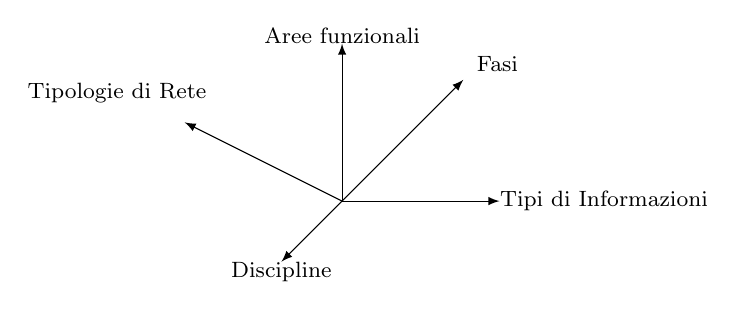
\begin{tikzpicture}
		\tikzset{mynode/.style={font=\footnotesize,inner sep=0pt,text=black}}
		%Begin plot
		\draw[-latex] (0,0,0) -- (2,0,0)node[mynode,anchor=west]{Tipi di Informazioni};
		\draw[-latex] (0,0,0) -- (0,2,0)node[mynode,anchor=south]{Aree funzionali};
		\draw[-latex] (0,0,0) -- (0,0,2)node[mynode,anchor=north]{Discipline};
		\draw[-latex] (0,0,0) -- (-2,1,0)node[mynode,anchor=north west,xshift=-2cm,yshift=0.5cm]{Tipologie di Rete};
		\draw[-latex] (0,0,0) -- (0,0,-4)node[mynode,anchor=north east,xshift=0.7cm,yshift=0.3cm]{Fasi};	
	\end{tikzpicture}
	\caption{Tipi di management.}
	\label{img:management_types}
\end{figure}\\
Come è possibile osservare dalla Figura \ref{img:management_types} vi sono vari tipi di management. Le \textit{aree funzionali} comprendono tutto ciò che riguarda configuration, performance, fault, security, accounting. Le \textit{fasi}, invece, planning, installation, operation, change, dismissing. Le \textit{tipologie di rete} comprendono internet, VPN, corporate, WAN, LAN, etc. Non esiste dunque un solo sistema di management e quindi non esiste una sola soluzione per il management, contando il fatto che non abbiamo parlato di organizzazione, fattori economici e legali, etc. Sostanzialmente l'idea fondamentale è quella di \textit{utilizzare concetti e formati standard per permettere l'interscambio di informazioni tra i fari livelli di management e tra le entità che lo compongono} (integrated management).

\noindent Vediamo adesso la \textit{management architecture}, ossia l'insieme degli standard relativi al management. Questa è suddivisa in:
\begin{itemize}
	\item \textbf{Information model}. Descrive il sistema sintattico e semantico per la rappresentazione delle risorse e delle informazioni in maniera orientata al management e indipendente dal venditore.
	\item \textbf{Communication model}. Descrive il sistema di accesso agli oggetti gestiti ed i protocolli di management.
	\item \textbf{Function model}. Organizza il sistema di management in sotto-task più gestibili e definisce funzioni di management generiche.
	\item \textbf{Organization model}. Definisce ruoli, modelli di cooperazione e domini di competenza.
\end{itemize}
L'unione dell'information e del communication model rappresenta gli \textquotedblleft elementi" hardware e software abbastanza comprensibili da un ingegnere, mentre l'unione di function ed organization model rappresenta gli \textquotedblleft elementi" organizzativi imprescindibili che coinvolgono persone e non macchine. Tutta questa architettura concorre a definire la \textbf{management platform}, che può (a volte) essere composta da elementi semplici, utilizzabili anche singolarmente (e.g. ping).

\noindent Per chi e perché viene attuato il management? In sostanza:
\begin{itemize}
	\item L'\textit{utente} finale è interessato ad avere un sistema affidabile, flessibile, sicuro, efficace, poco costoso, etc. e non è interessato a come viene realizzato. Tuttavia, le esigenze dell'utente sono alla base del management.
	\item L'\textit{azienda} vuole trarre profitti e anch'essa non è interessata a come un sistema viene realizzata. Tuttavia, anche le esigenze dell'azienda sono alla base del management.
\end{itemize}
Gli obiettivi del management devono dunque essere quelli di offrire all'utente il \textquotedblleft prodotto" (QoS, banda, whatever) richiesto e di gestire al meglio le risorse a disposizione evitando gli sprechi.

Una \textit{rete di telecomunicazioni} è progettata per offrire un servizio di comunicazione a distanza secondo modalità definite in un \textit{rapporto contrattuale}; quest'ultimo rappresenta la base del management. I soggetti coinvolti in questo rapporto sono sostanzialmente tre:
\begin{itemize}
	\item \textbf{Network operator}, cioè il gestore di rete. Si occupa di predisporre e di mantenere operativa l'infrastruttura necessaria al funzionamento dei servizi di telecomunicazioni utilizzando un supporto tecnico ed organizzativo. È sostanzialmente vincolato al rispetto dei requisiti di qualità per ognuno dei servizi supportati e di un costo di fornitura commisurato al beneficio ottenibile.
	\item \textbf{Service provider}, ossia il fornitore del servizio. Il service provider rende disponibili i servizi e le relative logiche di esecuzione che il cliente può personalizzare con modalità definite nei suoi impegni contrattuali (ivi compresi gli aspetti di qualità e costo). Utilizza inoltre le risorse dell'infrastruttura rese disponibili dal gestore di rete per trasferire l'informazione tra l'origine e la destinazione della comunicazione.
	\item \textbf{Service customer}, cioè il cliente che usufruisce del servizio.
\end{itemize}
Un \textit{servizio di telecomunicazione} è un servizio complesso che comprende: \textit{dispositivi terminali} (Terminal Equipment, TE) attraverso i quali l'utente usufruisce di uno o più servizi di telecomunicazione; \textit{dispositivi di accesso alla rete}; una \textit{rete} come piattaforma di connessione. Esso offre:
\begin{itemize}
	\item \textbf{Servizi applicativi}. Questi rispondono alle esigenze di comunicazione (in senso lato) degli utenti e comprendono, cioè, accanto alle problematiche connesse al trasferimento dell'informazione, anche aspetti legati all'utilizzazione finale.
	\item \textbf{Servizi di rete}. Rendono possibile il trasferimento dell'informazione tra due punti di accesso alla rete.
\end{itemize}
Generalmente abbiamo più \textit{tipologie di reti} di telecomunicazione, che si possono classificare in base a: \textit{profilo di utenza, mobilità dei terminali, estensione fisica, gamma dei servizi supportati}. La classificazione della rete aiuta a capire che tipo di management è necessario, quali tecnologie usare e, nel caso della sicurezza, è indispensabile per definire il \textit{Threat Model} visto in precedenza.

Per quanto riguarda le reti distinte in base al profilo di utenza abbiamo \textit{reti pubbliche} e \textit{reti private}. Nelle prime l'accesso è consentito a chiunque, previa stipulazione di un accordo contrattuale con il fornitore di servizi (e.g. Public Switched Telephone Network, PSTN). Nelle seconde gli utenti costituiscono un insieme chiuso ed omogeneo per quanto riguarda le esigenze di comunicazione e l'abilitazione all'accesso richiede la sottoscrizione di un accordo tra cliente e fornitore non assimilabile a quello definito in ambito pubblico (e.g. TErrestrial Trunked RAdio, TETRA).

Nelle reti distinte in base alla mobilità dei terminali, invece, abbiamo \textit{reti fisse}, \textit{reti mobili} e \textit{reti nomadiche}. Nelle prime i servizi supportati dalla rete sono accessibili solo da parte di utenti che non variano la propria posizione durante la comunicazione, oppure restano in un intorno limitato del punto di accesso alla rete; nelle seconde l'accesso è consentito ad utenti che non hanno alcun vincolo alla loro possibilità di movimento; nelle ultime, l'accesso è consentito ad utenti che non hanno alcun vincolo alla loro possibilità di movimento, ma durante la fruizione del servizio restano relativamente statici.

Per le reti distinte in base alla loro estensione abbiamo la \textit{rete in area locale} (Local Area Network, LAN), nelle quali l'area di interesse è limitata ad un singolo edificio o ad un complesso di insediamenti entro il raggio di qualche chilometro, la \textit{rete in area metropolitana} (Metropolitan Area Network, MAN) che fornisce servizi agli utenti che risiedono in una città o in una provincia, e le \textit{reti in area geografica} nelle quali gli utenti sono distribuiti su un'area molto estesa (una nazione, un continente, l'intero globo terrestre). Si noti che comunque questa classificazione non è più molto utile perché le tecnologie sono simili.

Infine, per reti distinte in base alla gamma dei servizi supportati abbiamo le \textit{reti dedicate ad un servizio} e le \textit{reti integrate nei servizi}. Le prime furono originariamente progettate e realizzate per offrire una sola tipologia di servizio (e.g. rete telegrafica/telefonica, rete per dati) e possono essere estese anche ad un insieme ristretto di altri servizi, pur con limitazioni severe per ciò che concerne la qualità conseguibile. Le seconde, invece, rendono possibile la fruizione di una vasta gamma di servizi di telecomunicazione con prestazioni di qualità e di costo superiori a quelli delle reti monoservizio.

La rappresentazione più intuitiva di una rete di telecomunicazione è data dal suo modello geometrico, ovvero dalla propria \textit{topologia}, nel quale gli elementi costitutivi sono i \textit{rami} e i \textit{nodi}. Un \textit{ramo} costituisce l'elemento di connessione di due nodi ed è rappresentato graficamente da un segmento \textit{orientato}, mentre un \textit{nodo} individua un elemento della rete connotato da specifiche funzionalità. Il significato di queste entità geometriche è diverso a seconda del tipo di operatività che si considera. Per gestire una rete è indispensabile conoscere la topologia della rete al giusto livello; si noti che non stiamo parlando di topologie a bus, anello, stella o altro.\\
Una rete esplica la funzione di trasferimento dell'informazione verso nodi preposti alla funzione di utilizzazione dell'informazione. In una rete si distinguono due sottoinsiemi di risorse funzionali dedicate al trasporto: \textit{rete logica} (svolge compiti di natura logica) e \textit{rete fisica} (svolge compiti di natura esclusivamente fisica). Le reti fisica e logica sono in stretta relazione gerarchica dato poiché le funzioni di natura logica utilizzano come supporto quelle fisiche e le funzioni di natura fisica sono al servizio delle altre. L'interazione tra rete fisica e rete logica segue il modello di interazione Client/Server in cui la rete logica agisce come Client e quella fisica come Server.\\
Una \textbf{rete logica} è un'infrastruttura che consente il trasferimento di informazioni da uno (o più) mittenti ad uno (o più) destinatari tra loro remoti e raggruppa funzioni di natura logica che hanno come obiettivo la la fornitura di un servizio di rete; nella formazione di un percorso logico nella rete sono coinvolti rami e nodi. Un \textit{ramo} individua un percorso diretto che l'informazione segue per essere trasferita da un punto all'altro e descrive gli apparati di rete che svolgono la funzione di multiplazione. Un \textit{nodo} individua il mezzo di scambio tra due o più rami che afferiscono ed è situato in corrispondenza degli apparati di rete che svolgono la funzione di commutazione. Ad esempio, se \textquotedblleft guardiamo" una rete a livello di indirizzi IP stiamo individuando una topologia logica che, tuttavia, potrebbe essere diversa a livello applicativo.\\
Una \textbf{rete fisica} è un'infrastruttura preposta al trasferimento dei segnali fisici che veicolano l'informazione. Sostanzialmente è la sede delle funzionalità di natura trasmissiva che coinvolgono tutti gli aspetti di propagazione del segnale ed è l'infrastruttura base a cui fa riferimento la rete logica. In questo caso, un \textit{ramo} individua il percorso fisico su cui avviene il trasferimento dei segnali e modella gli apparati trasmissivi presenti su quella tratta; un \textit{nodo} invece individua il punto di trasmissione e/o ricezione dei segnali ed è situato in corrispondenza dei terminali di ricetrasmissione. Dunque per \textit{rete fisica} si intendono ad esempio cavi, connettori, hub, switch etc. In generale le topologie della rete logica e della rete fisica non coincidono.

La rete si divide in più \textit{sezioni}: sezione di \textbf{accesso} (rete di accesso) e sezione \textbf{dorsale o interna} (rete di trasporto). La \textit{rete di accesso} consente agli utenti l'accesso alla rete con linea di utente individuale, può essere realizzata con svariati supporti fisici ed è la sede di di risorse indivise o, in altri casi, condivise; il punto di accesso alla rete comprende l'interfaccia utente-rete. La \textit{rete di trasporto} consente il trasferimento di informazione tra i nodi di accesso utilizzando eventualmente dei nodi di transito ed è la sede di risorse di trasferimento e di elaborazione condivise; ha come supporto una rete fisica generalmente a fibre ottiche. Nella pratica con il termine rete di accesso si indica la parte di rete destinata al collegamento fra la sede dei singoli utenti finali fino alla prima centrale di commutazione e più in generale al collegamento tra un utente e il suo provider; la rete di trasporto è la rete che distribuisce il traffico verso i vari provider.

\noindent Le informazioni che vengono scambiate all'interno di una rete sono di tre tipi:
\begin{itemize}
	\item \textit{Informazione di utente}. È il traffico che l'utente invia e riceve e per il quale è disposto a pagare (da qui il termine \textit{payload}, il traffico \textquotedblleft pagante"). Alcuni esempi: voce, suoni musicali, immagini, testi. L'informazione veicolata dalle reti di telecomunicazioni è sempre soggetta ad  un'operazione di \textit{codifica di sorgente/canale} che ne riduce la ridondanza e ne aumenta l'affidabilità in dipendenza dal mezzo trasmissivo. L'informazione di utente comprende anche l'informazione generata da una sorgente in relazione ad una specifica applicazione ed è destinata a uno o più collettori di informazione; può essere \textit{monomediale} (interessa un solo mezzo di rappresentazione) o \textit{multimediale} (coinvolge una pluralità di mezzi di rappresentazione). Genericamente è soggetta a QoS, ma la QoS richiesta è strettamente dipendente dal tipo di informazione e dall'utilizzatore (Human-Human, Human-Machine, Machine-Machine). L'informazione utente può anche essere soggetta a elaborazioni \textit{trasparenti} o \textit{apparenti} nel corso del trasporto.
	
	\item \textit{Informazione di segnalazione}. Costituisce quella parte di informazione che serve alla rete per funzionare in presenza di traffico di utente: è un traffico accessorio a quello utente che serve per far fluire l'informazione da una parte all'altra della rete in modo corretto (e.g. nel telefono: comporre un numero, individuare l'utente, inviare il numero del chiamante, etc.). Più precisamente possiamo dire che l'informazione di segnalazione (o di controllo) svolge una funzione di supporto per il corretto trasferimento dell'informazione di utente. Questo tipo di informazione è assente in caso di mancanza del traffico di utente. A livello pratico consente un'interazione tra cliente/utente e fornitore per:
		\begin{itemize}
			\item iniziare una comunicazione,
			\item negoziarne le caratteristiche qualitative e quantitative iniziali,
			\item modificare tali caratteristiche nel corso della comunicazione,
			\item aumentare le potenzialità dei servizi di base coinvolgendo le risorse di elaborazione che si rendono disponibili durante la comunicazione.
		\end{itemize}
	
	\item \textit{Informazione di gestione}. Costituisce il traffico che la rete produce per il suo normale e corretto funzionamento. Garantisce, cioè, il corretto svolgimento delle operazioni necessarie alla gestione delle risorse di rete relative all'erogazione dei servizi, al mantenimento del servizio, all'addebito del servizio. È necessario uno scambio di informazione di gestione tra le apparecchiature di rete e quelle terminali per un utilizzo efficiente dell'infrastruttura di rete. Esempi sono le tabelle di routing nel TCP/IP ed i keep-alive.
\end{itemize}
È importante ricordare che lo scopo di una rete è quello di trasportare la sola informazione dell'utente, tutto il resto (traffico di segnalazione e di gestione) costituisce \textit{overhead} ed occorre minimizzarlo.\\
Il trasferimento delle informazioni di utente, di segnalazione e di gestione può essere attuato sia nell'ambito di un'unica infrastruttura (come si preferiva in passato per le reti dedicate a un servizio) sia utilizzando infrastrutture separate in accordo alle impostazioni più moderne di integrazione dei servizi e di distribuzione dell'intelligenza all'interno della rete. In alcune reti, come SS7, informazioni di segnalazione e di gestioni sono logicamente separate dai dati; nei casi a canale comune è possibile sfruttare al meglio la banda totale del sistema, nei casi a canale separato si ha un maggior controllo del sistema poiché il canale di segnalazione e gestione non viene congestionato dalla trasmissione dati. A seconda del tipo di servizio che si vuole utilizzare funzionerà meglio uno o l'altro tipo. Si noti comunque che nel TCP/IP e nella rete Internet si usa un sistema di segnalazione e gestione a canale comune; nel caso di reti \textit{datagram oriented} l'informazione di segnalazione fa parte dell'header dei pacchetti (e.g. header IP).
\begin{figure}[htbp]
	\centering
	\includegraphics[scale = 0.55]{images/ISO-OSI}
	\caption{Modello ISO/OSI.}
	\label{img:ISO-OSI}
\end{figure}\\
In Figura \ref{img:ISO-OSI} è rappresentato il modello ISO/OSI. È importante sapere due concetti riguardanti questo modello: \textit{information hiding} (non esporre l'implementazione, ma solo un servizio) e \textit{separation of concerns} (non duplicare le funzionalità). La maggior parte dei problemi odierni del TCP/IP deriva dalla violazione di questi due concetti. Un problema fondamentale del modello ISO/OSI è dovuto al fatto che il traffico utente, di segnalazione e di controllo non possono separati e non vi è possibilità di fare il \textit{cross layer}, ovvero saltare da un layer all'altro. Un esempio di pila protocollare che permette di ovviare a questi problemi è una pila tridimensionale (e.g. ATM): a fianco dei layers dati vi è un unico layer di segnalazione, dietro ai quali vi è un unico layer di controllo.\\
Le reti wireless e wired che prenderemo in considerazione nel seguito sono 802.3 (ethernet), 802.11 (WiFi), 802.1 e LTE.
\begin{figure}[htbp]
	\centering
	\includegraphics[scale = 0.55]{images/network-devices}
	\caption{Dispositivi di rete.}
	\label{img:network-devices}
\end{figure}\\
I dispositivi che operano nelle reti ed in Internet (Figura \ref{img:network-devices}) sono differenziati in base al livello protocollare in cui operano. A livello fisico abbiamo \textit{repeater} (due porte) e \textit{hub} (più porte). A livello collegamento abbiamo i \textit{bridge} (connettono tecnologie diverse ma compatibili usando il Logical Link Control e cambiando un frame da un tipo ad un altro purché compatibili -- e.g. frame 802.11 in frame ethernet) e gli \textit{switch} (connette tecnologie uguali, instradando i pacchetti verso l'indirizzo desiderato). A livello rete abbiamo i \textit{router}, dispositivi che lavorano a livello di indirizzi IP e che decidono l'instradamento basandosi su tabelle e protocolli di apprendimento delle route. Ai livelli superiori si parla di \textit{gateway}. Il fatto che questi dispositivi siano dotati di \textquotedblleft intelligenza" (i.e. managed) non significa che operino a livelli superiori a quello di riferimento (e.g. uno switch managed opera sempre a livello 2, anche se presenta un'interfaccia di gestione web). Dato che il TCP/IP occupa i livelli 3 e 4, in Internet vi sono solo routers e gateways.

\section{Internet}
